\section{Data Distribution Service (DDS) as middleware}

DDS is a publish-subscribe standard by the OMG group and is available as open-source or commercial implementations like OpenDDS or RTI Connext. DDS supports topic, content or type based subscribing, where a topic is a somewhat arbitrary general naming of a message, content is certain properties evaluated at runtime of a message, and type is using a static type schema of a higher-level language, for example CSharp or Java, to distinguish messages. Because DDS is based on publish-subscribe, it provides a flexible and adaptable architecture, with a large number of configuration properties and ranging from one-to-one to many-to-many communication support.

\subsection{Infrastructure:, DLRL and DCPS}
The DDS infrastructure can be see in figure \ref{fig:DDSIinfrastructure}\footnote{\cite{Lopez-Vega2013}}. The Publish / Subscribe interface are connection points where nodes can communicate with each-other using a topic. The Quality of service (QoS) configuration is used to specify important parameters for the distributed application based on the given requirements. These QoS parameters can include destination ordering to ensure that messages always arrival in order. This is applied to each specific piece of data. The Topic based anonymous communication handles topics, so decoupled communication can happen.

\begin{figure}[H]
	\centering
	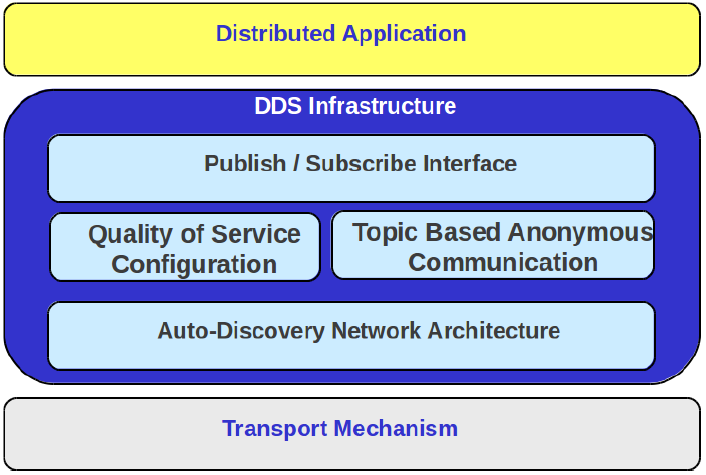
\includegraphics[scale=0.8]{middleware/DDSIinfrastructure.png}
	\caption{The Data Distribution Service Infrastructure.}
	\label{fig:DDSIinfrastructure}
\end{figure}

The Data Centric Publish Subscribe (DCPS) enables publishers and subscribers to exchange data items identified by a topic within a shared data-space also known as a domain. This allows a publisher who wants to update data content belonging to a topic. The middleware has the responsibility of delivering the update to the subscribers. The domain works as a distributed cache so data-caching and content-based-filtering can be accessed by the publishers and subscribers.

Within the DDS there also is a optional layer the Data Local Reconstruction Layer (DLRL) that allows for a more direct approach to the exchanged data, seamlessly integrated with the native-language constructs. It uses object orientation because of the benefits it provides in software engineering and therefore enables the application developers to use the underlying DDS features.

\subsection{DDS-SDP - Simple Discovery Protocol}
In the DDS we need a way to track the presence of all participants and endpoints in the system so when a new participant join, it will be able to discover new participants in the same Domain. This is possible because SDP allows to build peer-to-peer architectures without the need of any broker. 

\subsection{DDS-IS - The Interconnection Service}
The DDS data spaces Interconnection Service (DDS-IS) is capable of bridging DDS domains and adapting between different data schemes. DDS-IS has the following features: Scalability, data model compatibility and confidentiality, delivery guarantees, standard compliance and performance is good enough for use cases in need of the service. The three key features that DDS-IS is solving is system scalability, data transformation between data-spaces, and QoS adaptation between remote entities.\footnote{\cite{Lopez-Vega2013}}

The architecture of DDS-IS is straightforward. All components in need of a publish/subscribe service uses DDS as middleware. The difference between DDS and DDS-IS is that a DDS-IS node is added in-between two DDS domains which are not able to bridge directly to each-other, or would make a huge impact on performance if they did. In figure \ref{fig:DDSISarchitecture}\footnote{\cite{Lopez-Vega2013}} the architecture of DDS-IS can be seen. The impact on the standard DDS performance is very low and the DDS-IS improves the scalability of DDS systems by reducing the network traffic load between remotely interconnected data spaces.

\begin{figure}[H]
	\centering
	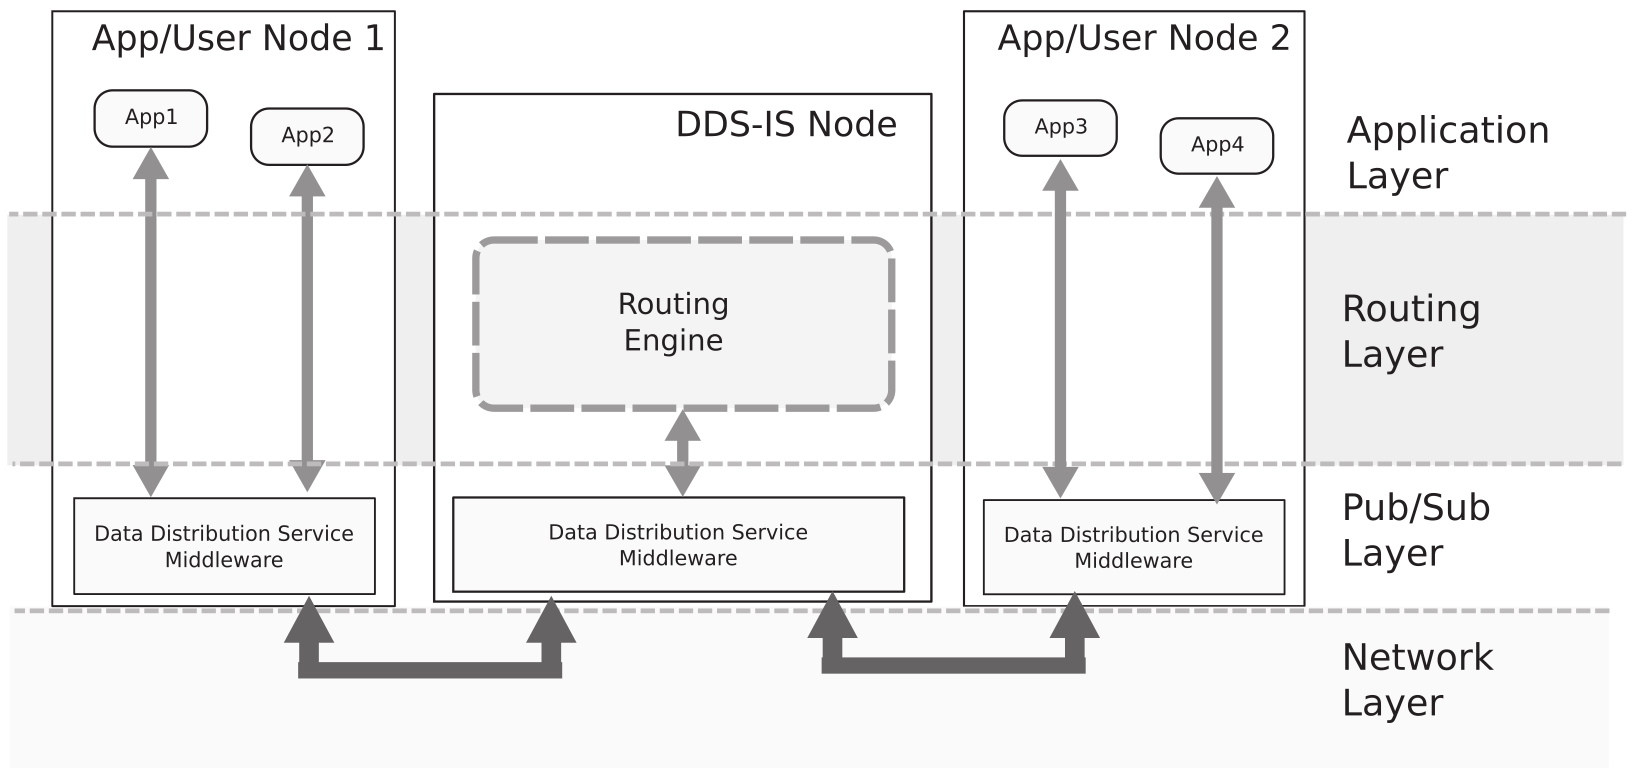
\includegraphics[scale=0.18]{middleware/DDSISarchitecture.png}
	\caption{Layered DDS-IS architecture}
	\label{fig:DDSISarchitecture}
\end{figure}
